\documentclass[Rapport/Rapport_main.tex]{subfiles}
\begin{document}
\section{Metode og Proces}
I dette afsnit beskrives processen af udarbejdelsen af applikationen CarnGo, et 4. semesterprojekt udarbejdet i samarbejdet med Aarhus Universitet. I forlængelse med dette, vil der være en beskrivelse af de redskaber og udviklingsmetoder, som er anvendt under arbejdsprocessen. Projektet har visse krav og læringsmål angivet af Aarhus Universitet: 
\begin{itemize}
    \item Anvende en iterativ udviklingsproces
    \item Anvende projekt- og versionsstyringsværktøjer
    \item Kombinere viden fra flere af semestrets kurser og anvende denne i projektet.
\end{itemize}
Et vital element for udviklingsprocessen er, at den er iterativ. Det er såvel et krav for projektet, men også en central del af softwareudvikling. Hvis planlægningen skal være statisk, kræver det stabile krav og en forudsigende arbejdsproces. Dette har vist sig at være en farlig antagelse for softwareudvikling\cite{fowler}. Projektgruppen har derfor valgt at anvende Scrum som udviklingsmetode\cite{Scrum}. 
Hvis der ønskes den fulde proces dokumentation, henvises læseren til bilag \textbf{Proces}. 

\subsection{Anvendelse af Scrum i PRJ4, Gruppe 5}
Til forskel for de tidligere semestre har der ikke været noget krav om udviklingsmetoder til projektet med den undtagelse, at der skulle anvendes en iterativ udviklingsproces. Det blev besluttet at anvende Scrum, da flere medlemmer af gruppen havde god erfaring med dets fleksible og adaptive tilgang til arbejdsprocessen i form af korte iterationer med effektiv feedback mekanisme, samt gruppen havde en tilpasset version af Scrum, udarbejdet i et af de tidligere semesterprojekter. \\\\
Alle iterationer af projektets udarbejdelse, har tilføjet elementer til gruppens anvendelse af Scrum - gennem stadierne er der blev gjort erfaringer og reflekteret over, hvordan gruppen optimerer arbejdsprocessen, samt stadigvæk sikre kvalitet. Figur \ref{fig:scrum_usage} illustrerer den endelige udviklingsmetode for projektgruppen. 
\begin{figure}[H]
    \centering
    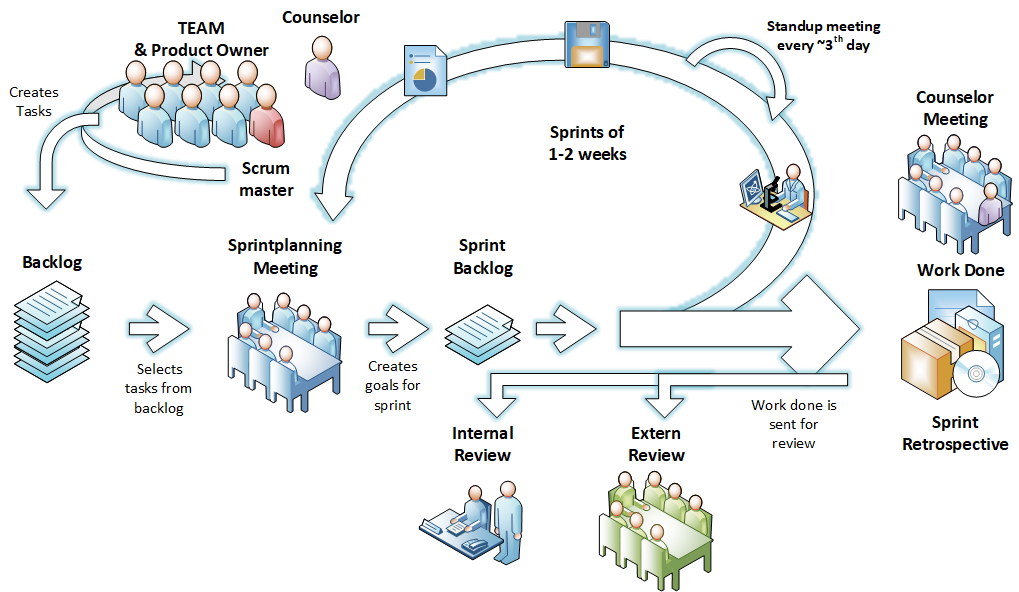
\includegraphics[width=\textwidth]{ProcesDokument/graphics/Scrum_usage.png}
    \caption{Anvendelse af Scrum i projektgruppe 5}
    \label{fig:scrum_usage}
\end{figure}
Gruppen har en Scrum Master, dog varetages rollen som productowner af hele gruppen: projektets krav er specificeret af gruppen. Gruppen vælger hvilke funktioner, egenskaber og arbejdsopgaver som skal prioriteres. Rollen som Scrum Master er tildelt Tristan Møller. Han har til ansvar at facilitere Scrum, fjerne interne og eksterne forhindringer og forbedre gruppens arbejdsproces. \\\\
Hvert sprint har en varighed af 1-2 uger, hvor der er Standup møder ca. hver 3. dag. Relevant opgaver tager fra Backlog'en og medtages i sprintplænlægningen - hvert gruppemedlem skal gerne have arbejdsopgaver svarende til 6-8 timers arbejde per uge. Den sidste mandag i sprintet reviewes alle substantielle eller kritiske tasks af et internt medlem. Desuden sendes materiale til review hos vejleder, hvis gruppen ønsker en vurdering udenfra. \\\\
Når et sprint er slut, tager gruppen et retrospektiv af sprintet. Her vurderes hvad som er gået godt, og hvilke processer som skal blive optimeret - i de seneres sprint blev der også foretaget en risikovurdering på projektets status.
Dette har været en af de mest essentielle feedback mekanismer i projektforløbet, og har gjort det muligt at forbedre gruppens arbejdsprocesser.

\subsection{Iterativ ASE-udviklingsmodel og SYSML}
I de forrige semestre har det været et krav at anvende ASA-modellen. Modellen er velegnet til software projekter for hvilke man har et godt domænekendskab. Den har dog flere elementer fra vandfaldsmodellen idet processerne er sekventiel\cite{ASE}. Scrum er en iterativ arbejdsmetode og der anvendes en iterativ tilgang ved udarbejdelse af alle processer i ASE-modellen (se figur \ref{fig:ASE}). Processerne beskrevet i ASE-modellen anvendes i flere iterationer (Sprints), hvor hver iteration ikke nødvendigvis er bundet til en proces: i et sprint kan der arbejdes på kravspecifikation og arkitekturen. 
\begin{figure}[H]
    \centering
    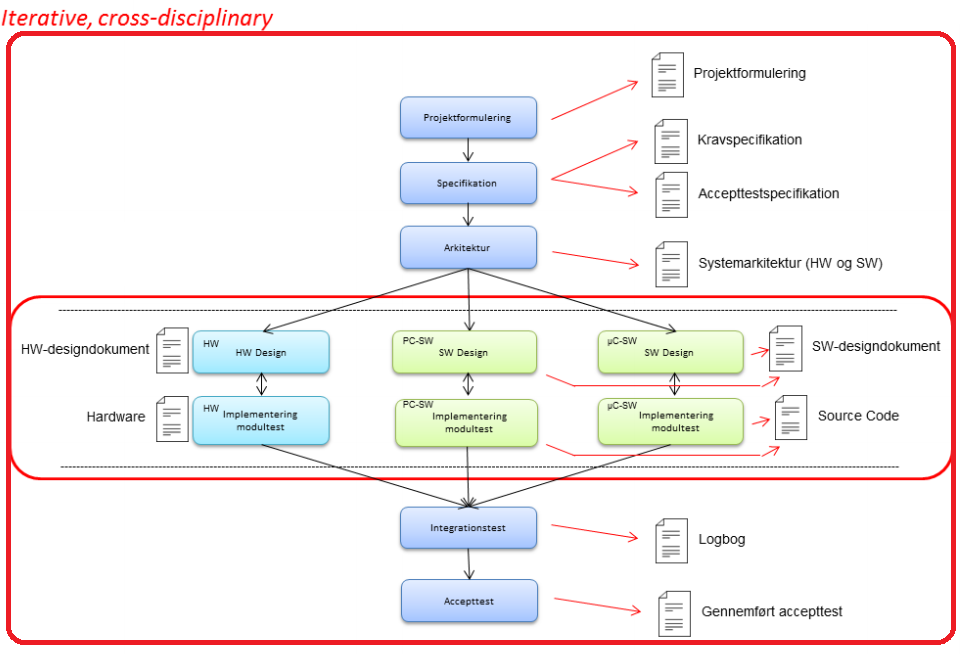
\includegraphics[width=\textwidth]{Rapport/Metode_og_Proces/grahpics/iterativASE.png}
    \caption{Iterativ ASE-model}
    \label{fig:ASE}
\end{figure}
Der anvendes SysML som analyse- og designreskab. Det bruges til at modellere og beskrive systemet. Af figur \ref{fig:Sysml_usage} ses de at Sekvens-, Statemachine- og Use Case-diagrammer bruges til at beskrive opførelsen af systemet. Class diagram fra UML er også inkluderet under struktur, da den beskriver strukturen af software samt relationen mellem de forskellige klasser. 
\begin{figure}[H]
    \centering
    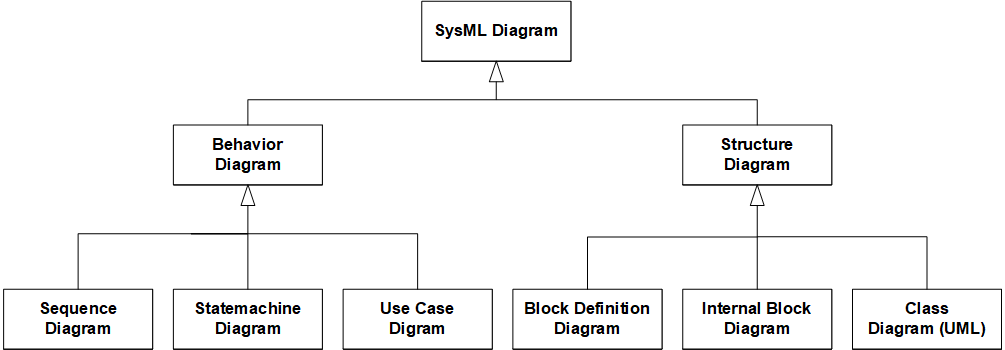
\includegraphics[width=\textwidth]{ProcesDokument/graphics/Sysml_usage.png}
    \caption{Anvendelse af SysML}
    \label{fig:Sysml_usage}
\end{figure}
Projektets udviklingsproces er nu defineret, samt modeller og redskaber som anvendes under udviklingen af systemet. Før systemet endeligt kan designes og implementeres, er det nødvendigt at foretage en analyse af systemet ud fra de givne krav.
\end{document}